% chktex-file 2
% chktex-file 8
% chktex-file 11
% chktex-file 24
% chktex-file 26
\chapter{Introduzione}
\label{cap:introduzione}
%\begin{figure}[h!]
%    \centering
%    \includegraphics[width=1\columnwidth]{img/quantum_entanglement.png}
%    \caption{Lorem}
%    \label{fig:entanglement}
%\end{figure}
%
%Introduzione al contesto applicativo.
%
%Lorem Figure \ref{fig:entanglement}
%
%Esempio di utilizzo di un termine nel glossario \gls{api}.
%
%Esempio di citazione in linea
%\cite{site:agile-manifesto}.
%
%Esempio di citazione nel pie' di pagina
%citazione\footcite{womak:lean-thinking}
%
%Termine di glossario \gls{apig}
%
%\lipsum[1-2]
\emph{In questo capitolo andremo ad enunciare la struttura del documento ed analizzeremo l'azienda ospitante stage curricolare e l'offerta proposta.}



\section{Profilo aziendale}

\myCompany (logo in figura \ref{fig:entanglement}) è un'azienda italiana specializzata nello sviluppo software e nella consulenza informatica. Da oltre quarant'anni, l'azienda si dedica alla riorganizzazione dei processi aziendali in diversi settori, progettando e implementando soluzioni digitali integrate. Con un forte orientamento verso l'innovazione, \myCompany si prefigge di contribuire al progresso delle aziende clienti, agevolandone la trasformazione digitale.

L'innovazione è il pilastro portante di \myCompany, che si impegna a essere costantemente riconosciuta come un'azienda altamente innovativa. L'azienda si distingue per la capacità di cogliere idee e suggerimenti provenienti da clienti, dipendenti e collaboratori, utilizzandoli come fonte di ispirazione per lo sviluppo di nuovi prodotti e soluzioni. Questo approccio si concretizza in un investimento significativo, pari al 15-20\% del fatturato annuo, destinato alle attività di Ricerca e Sviluppo, con una particolare attenzione agli aspetti sociali e alla riduzione dell'impatto ambientale.

Oltre all'innovazione, \myCompany è nota per l'eccellenza del servizio offerto ai propri clienti. La competenza dei suoi consulenti, maturata attraverso una solida esperienza pluriennale, consente all'azienda di proporre miglioramenti decisivi per rendere i processi aziendali dei clienti più efficaci ed efficienti.

La responsabilità ambientale è un altro elemento chiave per \myCompany. L'azienda ha intrapreso un percorso volto alla drastica riduzione delle proprie emissioni nocive, dimostrando un forte impegno verso la sostenibilità ambientale.

\myCompany conta oggi oltre 600 dipendenti e serve più di 2500 aziende. La sede principale è situata presso Villa Romanelli a Grisignano di Zocco, in provincia di Vicenza, nelle vicinanze dei Centri di Ricerca e Sviluppo e del Centro per la Formazione di Vicenza. L'azienda dispone inoltre di diverse filiali in Trentino-Alto Adige, Friuli-Venezia Giulia, Lombardia, Piemonte, Emilia-Romagna, Toscana, Campania e Puglia.

L'obiettivo principale di \myCompany è promuovere l'innovazione e il progresso tecnologico, sviluppando soluzioni software che rispondano alle esigenze dei clienti, garantendo al contempo la massima qualità e sicurezza. Eventuali ulteriori informazioni sono disponibili sul sito web dell'azienda\footnote{\url{https://www.sanmarcoinformatica.com/}}.
\begin{figure}[h!]
    \centering
    
\includegraphics[width=0.5\columnwidth]{img/logo_sanmarco_informatica.png}
    \caption{Logo di Sanmarco Informatica}
    \label{fig:entanglement}
\end{figure}
\subsection{Business Unit}
L'azienda è organizzata in \emph{Business Unit} (figura \ref{fig:business_unit}), centri di competenza specifici e autonomi, ma in costante relazione tra loro. Ciascuna \emph{Business Unit} è specializzata in un settore particolare ed è composta da team di sviluppo, consulenti e project manager, che collaborano per garantire la massima qualità e la piena soddisfazione dei clienti. \myCompany dispone di 10 \emph{Business Unit} principali:

\begin{itemize}
    \item \textbf{Jgalileo}: La soluzione di Enterprise Resource Planning (ERP) che ha reso celebre \myCompany. Jgalileo copre l'intero processo aziendale in modo integrato, permettendo di coordinare la filiera senza sprechi di tempo o risorse.
    \item \textbf{SMITech}: Specializzata nelle soluzioni per la Data Protection, SMITech offre servizi di Cybersecurity, gestione IBM Power, progetti di infrastruttura IT, e consulenza su Privacy e GDPR, migliorando la sicurezza e l'efficienza informatica delle aziende.
    \item \textbf{NextBI}: Questa \emph{Business Unit} si occupa di Business Intelligence, Performance Management e Customer Intelligence. La suite offerta da NextBI consente di gestire budget e controllo, analytics, simulazioni strategiche e di ottenere dati in tempo reale attraverso algoritmi avanzati e instant intelligence.
    \item \textbf{ECM}: Dedicata alla gestione della documentazione digitale, ECM fornisce strumenti per gestire l'intero ciclo di vita dei contenuti elettronici.
    \item \textbf{Discovery Quality}: Specializzata nella gestione della Governance Aziendale, del sistema della Qualità e dei processi aziendali. Discovery Quality coordina in modo proattivo e strutturato i diversi enti coinvolti, siano essi interni o esterni, e permette un monitoraggio continuo grazie a potenti strumenti di analytics.
    \item \textbf{Factory}: Dedicata alla Supply Chain e alle Operations nella fabbrica del futuro, Factory offre una suite di software per ottimizzare la gestione della produzione, migliorare il livello di servizio ai clienti, ridurre i livelli di scorta di magazzino e massimizzare i profitti riducendo i costi. Tra gli strumenti offerti figurano il Manufacturing Execution System (JMES), l'Advanced Planning \& Scheduling (APS) e il Supply Chain Collaboration (SCC).
    \item \textbf{JPA}: Questa \emph{Business Unit} è focalizzata sul Business Process Management (BPM), fornendo software per creare, gestire e automatizzare i processi aziendali. JPA consente di integrare e gestire i flussi di lavoro tra diverse aree funzionali e sistemi, riducendo il margine di errore e migliorando l'efficienza operativa.
    \item \textbf{JPM}: JPM è il software di Project Management sviluppato per supportare le aziende nella gestione dei progetti, facilitando il raggiungimento degli obiettivi di business. Offre strumenti avanzati per la pianificazione, l'esecuzione, il monitoraggio e il controllo dei progetti, accessibili da qualsiasi dispositivo.
    \item \textbf{4words}: Specializzata in e-commerce, sviluppo web e app, 4words offre servizi che vanno dalla realizzazione di siti web alla creazione di applicazioni mobili, fino al posizionamento sui motori di ricerca, supportando le aziende nel loro marketing digitale.
    \item \textbf{TCE}: La \emph{Business Unit} TCE è dedicata alla configurazione commerciale e tecnica, con un focus sull'ottimizzazione delle fasi di preventivazione e acquisizione degli ordini. Utilizzando la tecnologia CPQ (Configure Price and Quote), TCE permette alla forza vendite di configurare offerte personalizzate, automatizzando le complesse logiche commerciali e integrandosi con strumenti di disegno tecnico e renderizzazione 3D.
\end{itemize}

La \emph{Business Unit} di riferimento per lo stage è ECM (Enterprise Content Management), con sede presso il Centro per la Formazione di Vicenza. Questo team si occupa dello sviluppo e della manutenzione di servizi legati alla gestione dei documenti digitali, come ad esempio: la gestione documentale, Discovery XChange (per la conformità normativa sulla fatturazione elettronica), conservazione PEC integrata con Aruba, Digifinder (strumento per la ricerca di fatture elettroniche), Firmae (servizio di firma digitale dei documenti), e molti altri.

\begin{figure}[h!]
    \centering
    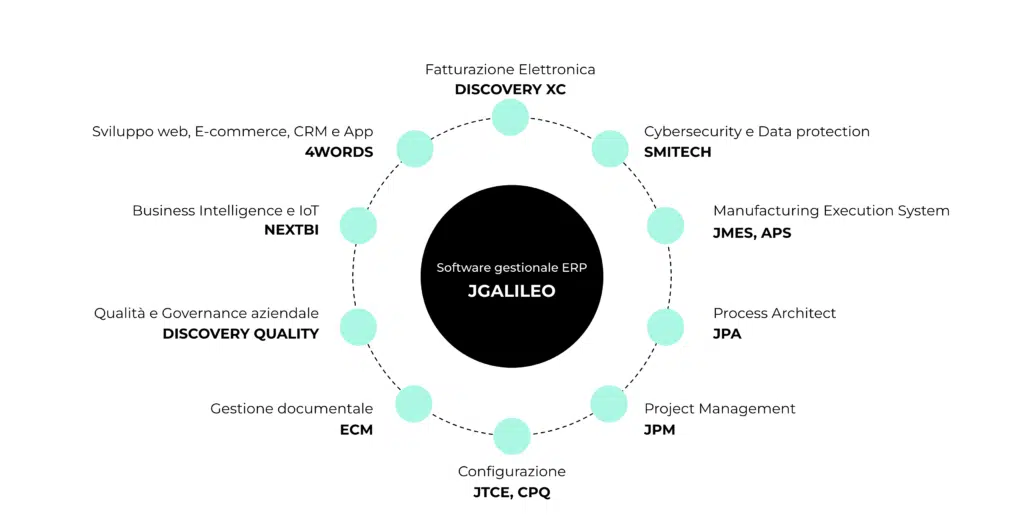
\includegraphics[width=0.8\columnwidth]{img/business_unit.png}
    \caption{Le Business Unit di Sanmarco Informatica}
    \label{fig:business_unit}
\end{figure}

\subsection{Metodologia di sviluppo}
La metodologia di lavoro, indipendentemente dalla Business Unit, è basata su un approccio \glsfirstoccur{\gls{agileg}} implementata con il framework \glsfirstoccur{\gls{scrumg}}. Agile è un approccio alla gestione dei progetti che si fonda su principi di collaborazione, auto-organizzazione e flessibilità. Scrum (figura \ref{fig:scrum}), in particolare, è un framework Agile che facilita la gestione di progetti complessi, garantendo la massima trasparenza e flessibilità. Questo viene realizzato suddividendo il progetto in sprint, ovvero periodi di tempo relativamente brevi in cui vengono fissati determinati obiettivi e attività.

Scrum si basa sull'idea che le decisioni si prendano in base a ciò che è noto al momento. Per questo motivo, la metodologia prevede tre principi fondamentali:

\begin{itemize}
    \item \textbf{Trasparenza}: Il team deve utilizzare un linguaggio comune e ben definito, per evitare dubbi e incomprensioni.
    \item \textbf{Ispezione}: Gli avanzamenti del progetto vengono ispezionati frequentemente per assicurarsi che il prodotto rimanga conforme ai requisiti e non si discosti dagli obiettivi.
    \item \textbf{Adattamento}: Se vengono rilevate discrepanze, il team deve essere in grado di adattarsi rapidamente, modificando le parti non conformi del prodotto per ridurre al minimo lo scarto rispetto agli obiettivi stabiliti. Questo processo avviene durante momenti specifici come lo Sprint Planning Meeting, il Daily Scrum e lo Sprint Review.
\end{itemize}

Il ciclo di sviluppo Scrum è strutturato in sprint, che sono iterazioni brevi, solitamente di durata variabile tra una e quattro settimane. Ogni sprint inizia con un meeting di pianificazione (\textit{Sprint Planning Meeting}), durante il quale il team di sviluppo esamina il lavoro svolto nello sprint precedente e definisce i nuovi obiettivi. Gli obiettivi fissati per uno sprint non possono essere modificati durante la sua esecuzione. Al termine dello sprint, il team presenta al committente una versione funzionante del prodotto, che include i progressi realizzati.

Per ogni sprint, i requisiti vengono estratti dal \textit{Product Backlog} e inseriti nello \textit{Sprint Backlog}, dove vengono suddivisi in task (o ticket), ciascuno dei quali rappresenta un'unità di lavoro da completare in un giorno.

Per garantire la fattibilità del prodotto e mantenere un'organizzazione ottimale, Scrum prevede una serie di eventi regolari:

\begin{itemize}
    \item \textbf{Sprint Planning Meeting}: All'inizio di ogni sprint, il team di sviluppo si riunisce per selezionare il lavoro da svolgere e definire il tempo necessario per ogni requisito del \textit{Product Backlog}.
    \item \textbf{Daily Scrum}: Durante lo sprint, il team si incontra quotidianamente per un breve meeting di massimo 15 minuti, in cui si discute del lavoro svolto, di quello previsto per la giornata successiva e degli eventuali problemi riscontrati.
    \item \textbf{Sprint Review}: Alla fine dello sprint, il team si riunisce con il committente per esaminare i cambiamenti nei requisiti, valutare il lavoro svolto e discutere delle problematiche riscontrate. Questo incontro è fondamentale per generare nuove idee e migliorare il prodotto, contribuendo alla pianificazione dello sprint successivo.
\end{itemize}

Ogni team Scrum è strutturato per essere indipendente, con l'obiettivo di ottimizzare i feedback ricevuti dal committente. Il team è generalmente composto da tre ruoli principali:

\begin{itemize}
    \item \textbf{Product Owner}: La persona che commissiona il progetto, segue lo sviluppo del prodotto e ne definisce i requisiti.
    \item \textbf{Team di sviluppo}: Il gruppo di professionisti che lavora alla realizzazione del prodotto.
    \item \textbf{Scrum Master}: La figura responsabile di mantenere il team di sviluppo focalizzato e motivato, proteggendolo da distrazioni e ponendo sfide che favoriscano il miglioramento continuo. Questo ruolo è spesso distinto dal Project Manager.
\end{itemize}

\begin{figure}[h!]
    \centering
    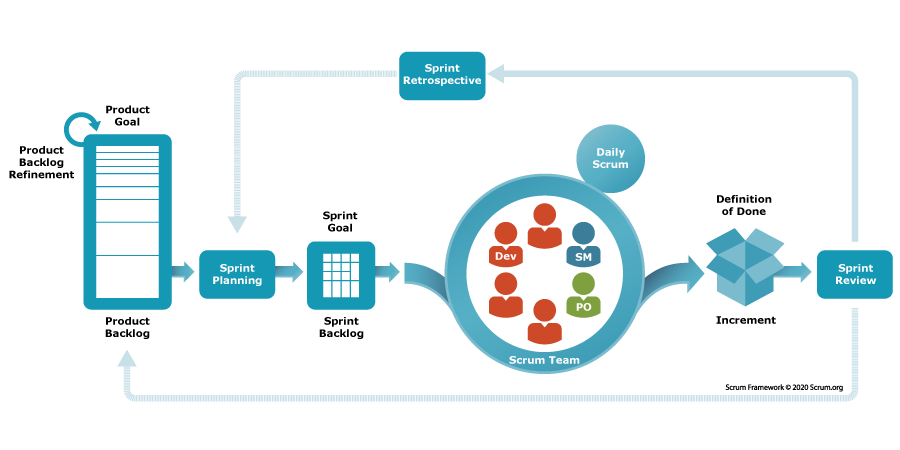
\includegraphics[width=0.9\columnwidth]{img/scrum.png}
    \caption{Framework Scrum}
    \label{fig:scrum}
\end{figure}

\section{L'offerta di stage}
L'obiettivo dello stage consiste nello sviluppo di un sistema avanzato per la catalogazione delle Poste Elettroniche Certificate (\glsfirstoccur{\gls{pecg}}), integrando tecnologie di Intelligenza Artificiale (\glsfirstoccur{\gls{aig}}) per migliorare l'efficienza e l'accuratezza del processo.

Il progetto è stato proposto dall'azienda in occasione dell'evento Stage IT 2024, organizzato dall'Università degli Studi di Padova e promosso da Confindustria Veneto Est. Questo evento mira a facilitare l'incontro tra studenti e aziende, offrendo la possibilità di svolgere uno stage formativo con particolare riferimento al settore \glsfirstoccur{\gls{ictg}}.

Gli obiettivi specifici del progetto sono i seguenti:

\begin{itemize}
    \item \textbf{Catalogazione Automatica Potenziata dall'IA}: Implementare modelli di apprendimento automatico che analizzino il contenuto delle PEC importate e le classifichino automaticamente in base al contenuto. L'Intelligenza Artificiale sarà in grado di rilevare informazioni quali mittente, destinatario, data e argomento, migliorando significativamente l'efficienza del processo di catalogazione.
    
    \item \textbf{Integrazione con un Sistema di Gestione Documentale}: Le informazioni estratte dalle PEC saranno integrate con un sistema di gestione documentale (DocuWave). Questo permetterà di persistere le email nel sistema, creando i metadati necessari con le informazioni estratte e collocandole nella corretta categoria di appartenenza.
    
    \item \textbf{Adattamento e Apprendimento Continuo}: Saranno implementati algoritmi di IA in grado di adattarsi e apprendere continuamente dai dati, migliorando le prestazioni del sistema nel tempo. Questo processo includerà l'ottimizzazione dei modelli di apprendimento automatico in base all'esperienza acquisita e ai feedback degli utenti.
    
    \item \textbf{Utilizzo dei Servizi Cloud AWS}: Il progetto prevede l'utilizzo dei servizi cloud offerti da Amazon Web Services (AWS) per l'addestramento del modello di apprendimento automatico scelto e per l'erogazione del servizio. L'infrastruttura necessaria sarà configurata direttamente sul cloud AWS per garantire scalabilità ed efficienza.
\end{itemize}

\section{Organizzazione del testo}

\begin{description}
    \item[{\hyperref[cap:descrizione-stage]{Il secondo capitolo}}] descrive lo stage, l'organizzazione, gli obiettivi e le attività svolte.
    
    \item[{\hyperref[cap:tecnologie]{Il terzo capitolo}}] approfondisce le tecnologie utilizzate oltre che gli strumenti e le metodologie di lavoro.
    
    \item[{\hyperref[cap:progettazione-codifica]{Il quarto capitolo}}] approfondisce la progettazione e la codifica del progetto.
    
    \item[{\hyperref[cap:sviluppi-futuri]{Il quinto capitolo}}] descrive i possibili sviluppi futuri del progetto.
    
    \item[{\hyperref[cap:conclusioni]{Il sesto capitolo}}] descrive le conclusioni del lavoro svolto.
\end{description}